\documentclass{tufte-handout}
\usepackage{graphicx}
\graphicspath{ {./images/} }

\title{Linear Models of Classification}
\author{Andres Ponce}
\begin{document}
\maketitle
\begin{abstract}
	The goal with \textbf{classification} is "to take 
	an input vector $x$ and to assign it to one of $K$
	discrete classes.
\end{abstract}

If we want to classify a certain input vector, we would have 
to map it to a certain region of a plane, defined by certain 
boundaries.\footnote{Is this similar to \textbf{linear programming},
where we had to optimize a linear combination of the parameters?}

If there are $D$ varaiables we are trying to optimize, then our 
answer will exist in a $D$ dimensional space. 
\subsection{Discriminants}
\textbf{Linear} discriminants can be of the form\footnote{Here, 
$w$ is the parameters, and $w_{0}$ is the bias.}
\[ y(x) = w^{T}x + w_{0}\]
We also ahve a \textbf{decision boundary}, where we know which of the
$K$ categories our input belongs to given our discriminant function,
and a certain cutoff value $C_{x}$.

We can also use a Bayesian approach to determine classification, if we 
calculate $p(C_{k}|x)$\footnote{The probability that given input $x$, 
it belongs in class $k$.}
\begin{marginfigure}
	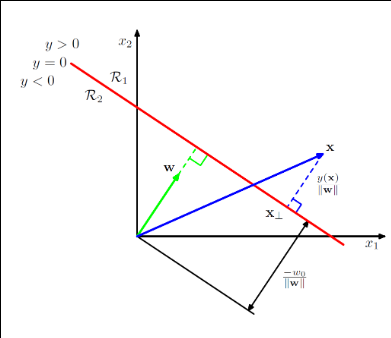
\includegraphics[width=\linewidth]{dec_boundary}
	\caption{The dotted green and blue lines are the 
		distance between the arbitrary point and the 
		decision boundary.}
\end{marginfigure}

How do we extend a linear discriminant to other classes? We can have
\textbf{One-vs-the-rest} or \textbf{one-vs-one} qualifiers.
\subsection{One-vs-the-rest}
	With this type of classifier functions, we try to distinguish those
	inputs on a binary case by case basis. That is, we try to one at a time
	build a classifier that knows points in $C_{i}$ from those points in other
	classes. However, when two points  "not in their repsective classes" fall
	in the same area, this area would be defined differently by the areas we're 
	actually testing.
	\begin{marginfigure}
		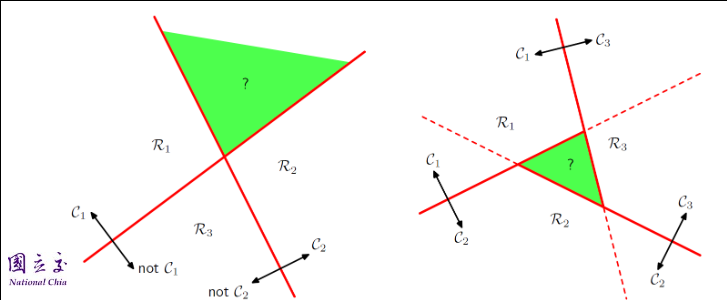
\includegraphics[width=\linewidth]{ambiguous}
		\caption{When a point is not in a certain region, it can 
			be ambiguous where it falls, if the same point can be thought
			of differently by each region.}
	\end{marginfigure}
\subsection{K-class discriminant}
	If we use $K$ linear functions of the form 
	\[ y_{k}(x) = w^{T}_{k}(x) + w_{k0}\]
	 
\end{document}
